\documentclass{article}
\usepackage{graphicx}
\usepackage{amsmath}
\usepackage{bbm}
\usepackage{natbib}
\usepackage[margin=1in]{geometry}
\usepackage{caption}

\title{BIOS 735 Project Proposal}
\author{Abby Foes, Zheng Lan, Justin Landis, Yu Liu, Alec Reinhardt}
\date{March 2025}

\begin{document}

\maketitle

\section{Introduction}

\subsection*{Data Description}

\noindent We identified a dataset for pasta sales from an Italian grocery store from January 2014 to December 2018. The dataset contains 116 time series with 1798 time points each, including the quantity of sales for specific pasta items and whether or not a promotion was placed on each item. The time series are hierarchical, with 4 brands and up to 45 unique items per brand (see Table \ref{tab:tab1}). Based on some preliminary data analysis, there is evidence of common temporal patterns in items sales within each brand, as well relationships between promotions and sales (see Figure \ref{fig:fig1}).

\vspace{1cm}

\begin{figure}[h]
    \centering
    \begin{minipage}{0.4\textwidth}
        \centering
        \begin{tabular}{c|c}
            \hline
            Brand & n \\
            \hline
            B1 & 42 \\
            B2 & 45 \\
            B3 & 21 \\
            B4 & 10 
        \end{tabular}
        \caption{Number of items within each pasta brand}
    \label{tab:tab1}
    \end{minipage}
    \hfill
    \begin{minipage}{0.5\textwidth}
        \centering
        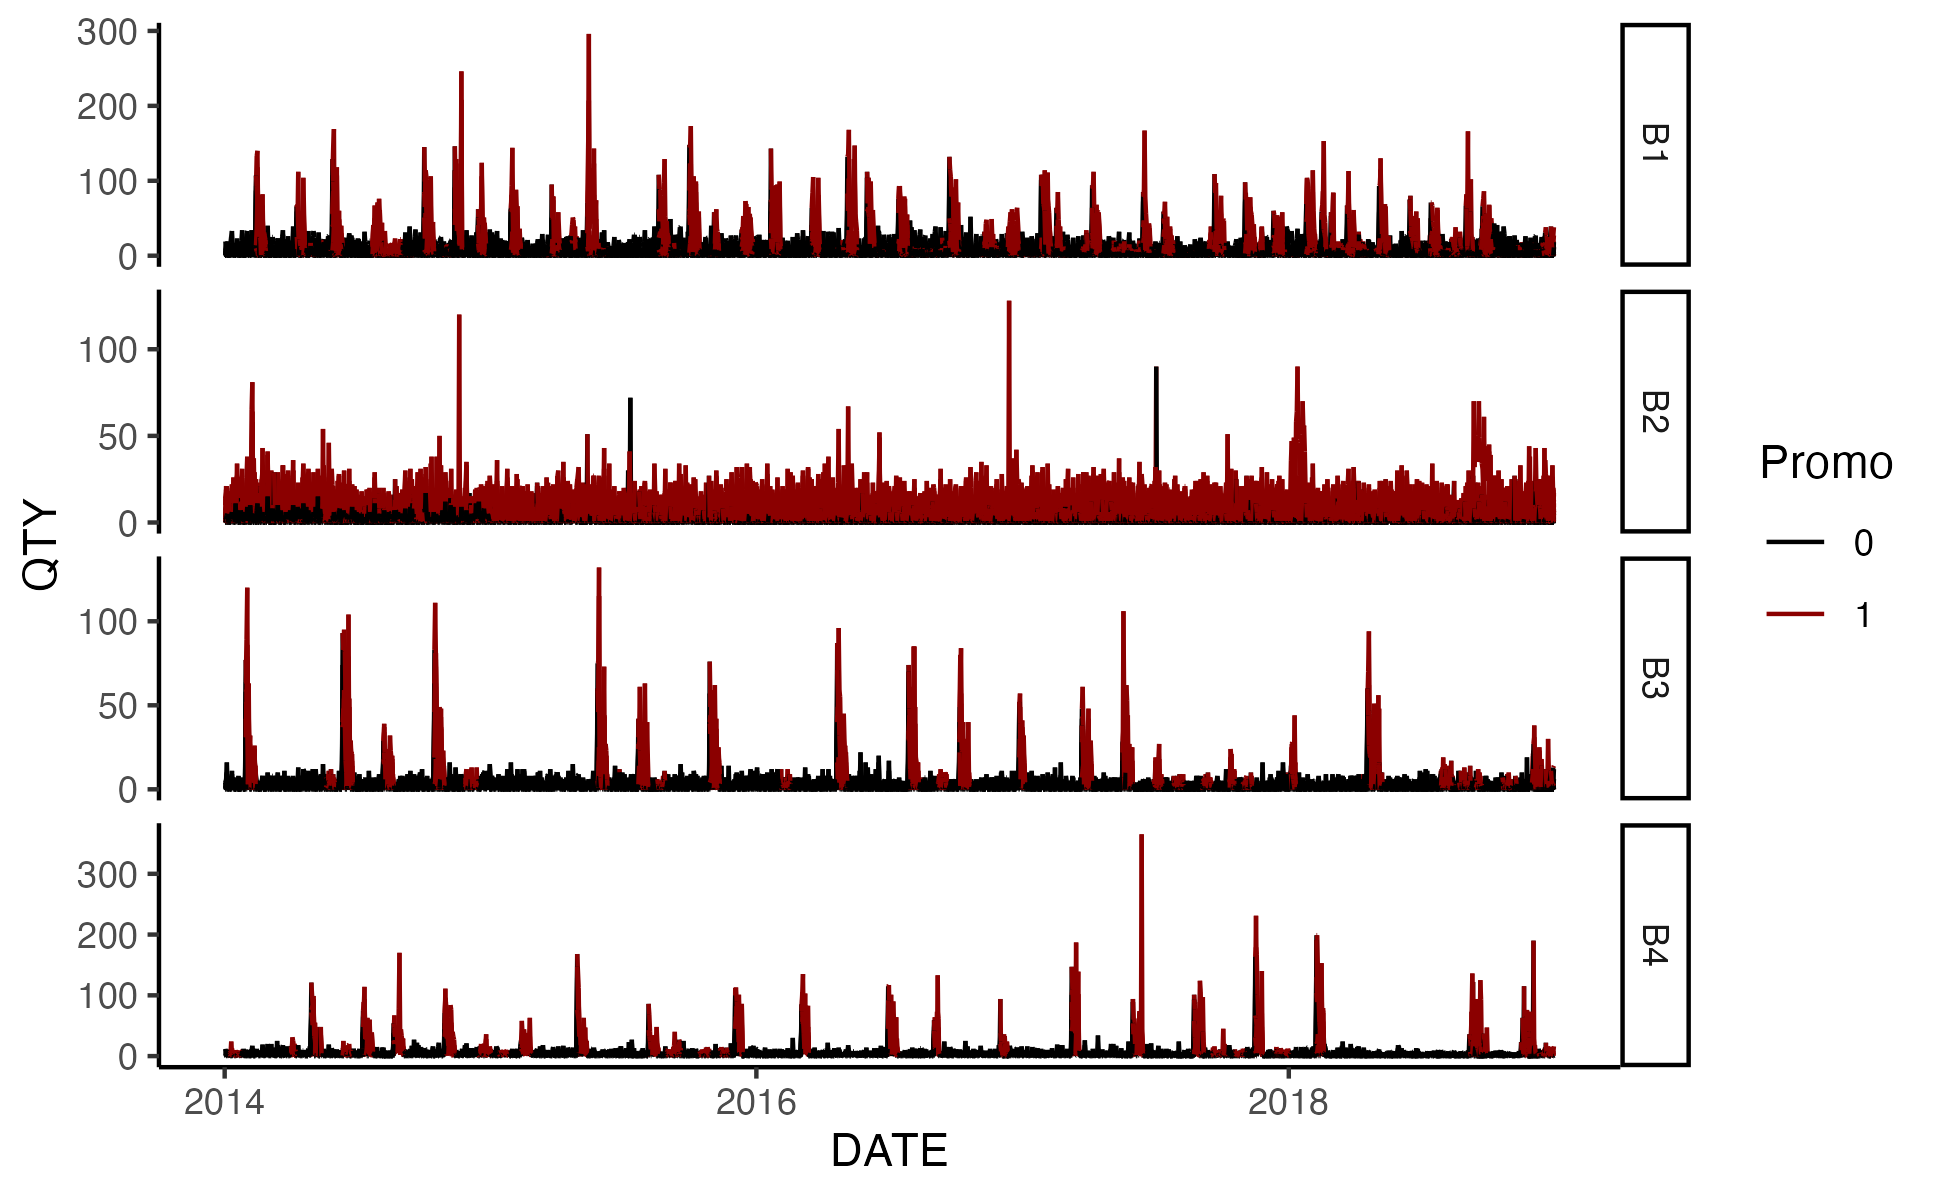
\includegraphics[width=\linewidth]{promotion_time_series.png} % Replace with your image file
        \caption{Time series of pasta sales per brand and item. Red lines indicate dates in which that brand's item was promoted}
        \label{fig:fig1}
    \end{minipage}    
\end{figure}

\subsection*{Research Questions}
\noindent We will consider the following questions: 

\begin{itemize}
    \item Can we improve forecasting accuracy by accounting for the hierarchical structure in the data, compared with modeling each brand and item independently? What about models that account for sparsity (for items with many days of no sales) or periodicity?
    \item How do temporal trends, and promotion-sales relationships, vary across pasta brands? Which points in time show the largest deviations? Is there evidence of periodic (seasonal) trends, and how do these relate across brands and items?
\end{itemize}

\vspace{1cm}

\section{Methods}

\subsection*{Notation}
\noindent{}We have $i = 1, 2, \dots, n$ items, $h = 1, \dots , m$ brands, and $t = 1, 2, \dots, T$ time points. Let $y_{hi,t}$ be the number of sales of item $i$ in brand $h$ at time $t$ and $x_{hi,t}$ the (binary) promotion.

\subsection*{Models}

\noindent To develop a forecasting model, we will adapt various classical approaches for time series modeling. For instance, the autoregressive model (AR) (see, e.g. \cite{box2015time}) assumes that the current outcome depends linearly on the previously observed outcomes (up to a certain lag $q$), covariates, and a noise term. This can be expressed as

\begin{align}
    & y_t = \alpha_0+\sum_{l=1}^q \beta_l y_{t-l} + \gamma x_{t} + \epsilon_{t}
    %& \epsilon_t \sim N(0,\sigma^2)
    \label{eq:model1}
\end{align}

\noindent where $y_t$ is the outcome at time point $t$, $\alpha_0$ is the population intercept, the $\beta_l$ terms capture the dependence between $y_t$ and previous time points, $\gamma$ captures the effect of (time-varying) covariate $x_t$ on $y_t$, and $\epsilon_t$ is the noise term, assumed to be mean zero Gaussian. As a first step, we plan to fit these models for each brand and item independently. The R package {\it astsa} utilizes model fitting methods such as Burg's Algorithm and Yule-Walker equations. However, we plan to also implement a MLE-based approach. Chapter 2 of the book (\cite{funatogawa2018longitudinal}) details the likelihood and steps for MLE for AR models.

\noindent In order to capture shared patterns among items within each brand, we propose a mixed effects AR model (see \cite{nicholls2012random} for example) of the form

\begin{align}
    & y_{hi,t} = (\alpha_0+a_h)+\sum_{l=1}^q (\beta_l+b_{h,l}) y_{hi,t-l} + (\gamma+g_h) x_{hi,t} + \epsilon_{t}     \label{eq:model2} \\
    & \alpha_h \sim N(0,\sigma_{\alpha}^2), \ b_{h,l} \sim N(0,\sigma_{\beta}^2), \ g_h \sim N(0,\sigma_{\gamma}^2), \ \epsilon_t \sim N(0,\sigma_{\epsilon}^2) \notag
\end{align}

\noindent where we introduce random intercept $a_h$, and random slopes $b_{h,l}$ and $g_h$ for the effects of previous timepoints and covariates, respectively. We assume that each term comes from a common distribution specific to each brand, in effect pooling information across items within each brand while still allowing for deviations. We will also consider simplifications and possible extensions of the above model, including modeling cross-brand dependencies. For model fitting, we will consider a Bayesian variation of Model \ref{eq:model2}, with suitable priors for model coefficients and residual noise. We will implement a Markov Chain Monte Carlo (MCMC) algorithm to sample the posterior of model parameters, which in turn allows for both prediction and uncertainty quantification (e.g. credible intervals).


Other competing approaches we plan to try include extensions of AR, such as ARMA and SARIMA (which can account for periodic trends), and alternatives like Hidden Markov Models.

\vspace{0.5cm}

\noindent {\bf Moving Average Model}
\begin{align*}
   & Y_{i,t} = \alpha + \epsilon_{i,t} +\sum_{j=1}^q\theta_i\epsilon_{i,t-j}
\end{align*}

\noindent {\bf ARMA Model}
\begin{align*}
    & y_t = \alpha + \sum_{l=1}^p\beta_l y_{t-l} + \gamma x_t+ \epsilon_t +\sum_{s=1}^q \epsilon_{t-s} \theta_{s}
    \\ &\epsilon_t\overset{i.i.d.}{\sim} N(0,\sigma^2)
\end{align*}






\vspace{1cm}

\subsection*{Analysis Plan}
\noindent We plan to fit the AR model described above and its variations using both a MLE-approach (using EM or NR algorithm) and with MCMC. For each model we fit, we will consider both non-hierarchical models, fit to each item independently, and a hierarchical variation which includes brand-specific model parameters (i.e. mixed effects model). Lastly, we will fit a machine learning approach such as Random Forest or Hidden Markov Models with off-the-shelf packages. 

To evaluate predictive performance, we will implement a holdout prediction scheme. The first $K$ timepoints will be used for model training, and we will assess prediction (with RMSE, e.g.) on the remaining timepoints. We will vary the size of $K$ to see how fast prediction improves as the amount of training data increases for the various models.

To address our set of questions, we will explore and interpret the different coefficient estimates for various models, after fitting to the entire dataset. In particular, the MCMC approach allows for natural quantification of uncertainty for both model coefficients and the predicted sales outcome, allowing to track where in time the different brands have evidence of significant differences. We will assess periodic trends with exploratory data analysis and by assessing goodness-of-fit for AR-based models that account for periodicity (e.g. SARIMA).



\bibliographystyle{apalike}
\bibliography{ref.bib}
\end{document}
